\documentclass[11pt,norsk]{article}

\usepackage[utf8]{inputenc}
\usepackage[T1]{fontenc,url}
\usepackage[norsk]{babel}
\usepackage{parskip}
\usepackage{lmodern}
\usepackage{microtype}
\usepackage{verbatim}
\usepackage{amsmath, amssymb}
\usepackage{mathtools}
\usepackage{tikz}
\usepackage{physics}
\usepackage{algorithm}
\usepackage{algpseudocode}
\usepackage{listings}
\usepackage{enumerate}
\usepackage{graphicx}
\usepackage{float}
\usepackage{epigraph}
\usepackage{hyperref}
\usepackage[toc,page]{appendix}
\usepackage{varioref}
\usepackage{enumitem}
\usepackage{siunitx}



% varioref stuff from Anders
\labelformat{section}{section~#1}
\labelformat{subsection}{section~#1}
\labelformat{subsubsection}{paragraph~#1}
\labelformat{equation}{(#1)}
\labelformat{figure}{figur~#1}
\labelformat{table}{table~#1}


\begin{document}



\title{FYS1210 - Prosjektoppgave i biologisk impedans}
\author{
	\begin{tabular}{rl}
        Jonas Gahr Sturtzel Lunde & (\texttt{jonassl})\\
	Bjørg Vårli Håland & (\texttt{bjorgvh})\\
	Linus Ekstrøm & (\texttt{linuse})
	\end{tabular}}
\date{}
\maketitle



\begin{figure}[H]
\centering

\includegraphics[width=0.5\textwidth]{fig/uio.png}
\end{figure}

\vfill


\pagebreak

\tableofcontents
\pagebreak



\section{Introduksjon}
I denne rapporten skal vi studere impedans hos levende og dødt vev, ved å se på potensialforskjeller mellom elektroder festet forskjellige steder på kroppen. Vi skal se på potensialforskjellene kroppen skaper under forskjellige ytre stimuli, og se hvordan vi kan bruke disse målingene til å studere hjerterytme og muskelspenning.


\section{Teori og bakgrunn}
\subsection{Admittans og impedans}
Impedans er et motstanden mot vekselstrøm, og måles i ohm. Vi kan dele impedans i en kompleks og en reell del, der den komplekse kalles reaktans, og den reelle resistans. Resistans er en direkte motstand mot all elektrisk bevegelse, proporsjonal med spenningen. Den er ved ren likestrøm gitt ved Ohms lov som
\begin{align}	R = U/I
\end{align}
der $U$ er spenningen i Volt, og $I$ er strømmen i Ampere. Resistansen måles i Ohm.

Reaktans er en frekvensavhengig motstand mot elektrisk bevegelse. Levende og dødt vev har utelukkende kapasitiv reaktans, som er invers proporsjonal med frekvens. Denne kapasitive reaktansen er gitt som
\begin{align}	X_C = -\frac{1}{2\pi f C}
\end{align}
der $C$ er kapasitansen, målt i Farad, og $f$ er frekvensen til signalet, i Hertz.

Disse motstandene mot elektrisk bevegelse kombineres i det vi kalles impedans. Deres effekt står $90^\circ$ på hverandre, og vi definerer impedansen som
\begin{align}	Z = R + iX
\end{align}

Den inverse av impedans kalles admittans, og viser materialets ledningsevne ved
\begin{align}	Y = 1/Z = \frac{1}{R + iX} = G + iB
\end{align}
Der vi har introdusert konduktansen G og suseptansen B. Admittans måles i siemens. 


\subsection{Elektroder}
Vi skal benytte oss av små elektroder, som består av en overgang mellom sølv/sølvklorid-metall og en gel med klorioner. Dette gir oss en overgang mellom ionisk og elektronisk ledning.

Når vi fester to elektroder på armen, måler vi på huden under i serie, noe som gir oss en biopolar måling. 

\begin{figure}[H]
\centering
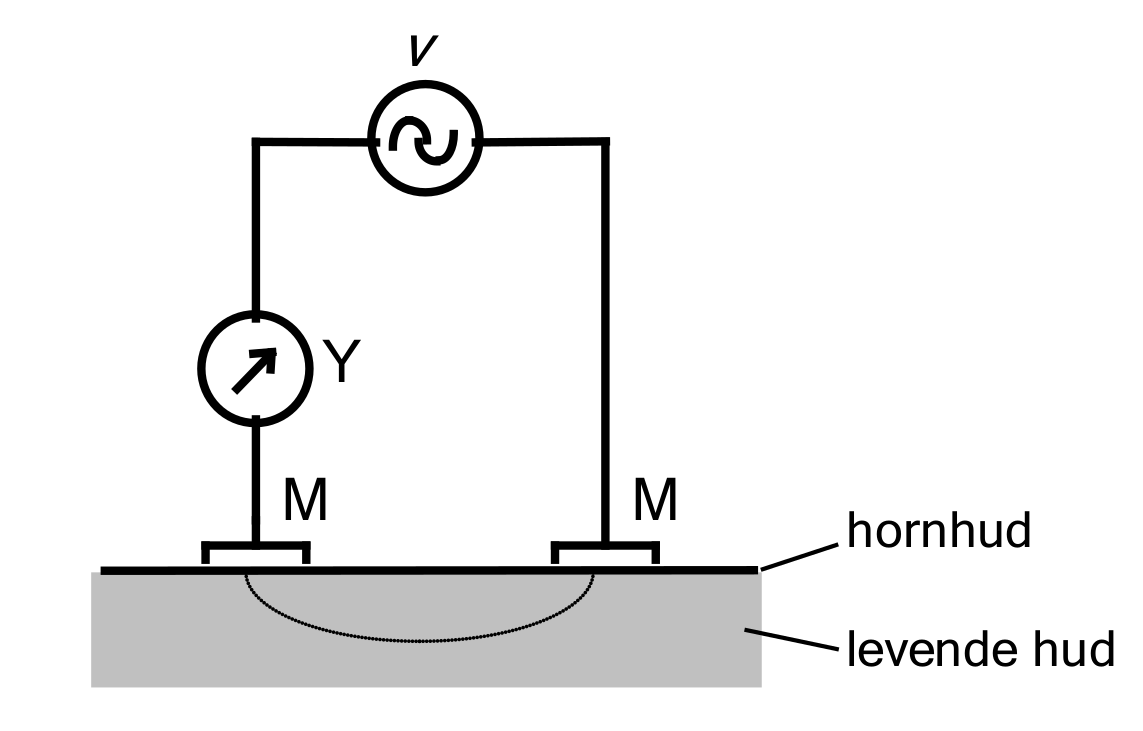
\includegraphics[width = 0.6\textwidth]{fig/screenshot1.png}
\caption{To-elektrodesystem på hud. Hentet fra oppgaveteksten.}
\end{figure}

Dersom vi heller ønsker å måle unipolart, kan vi endre størrelsen på den ene elektroden til å være 1/100 av den andre. Dersom det går strøm gjennom elektrodene vil strømtettheten - og dermed også spenningsfallet - bli mye høyere ved den minste elektroden (se \cite[Grimnes og Martinsen, s.~39]{BioImp}). I praksis vil det kun være denne som bestemmer effekten, og den andre blir nøytral. Vi måler dermed bare på det ene hudområdet. Dersom det ikke går strøm har størrelsen på elektrodene ingenting å si.

En annen måte å innføre unipolar måling på, er ved en tredje elektrode samt en operasjonsforsterker. Den tredje elektroden fungerer da som en referanseelektrode. Denne vil ha samme verdi som elektrode C, og vi kan dermed nøytralisere bidraget derfra. Hele målspenningen kommer nå fra elektrode M, og vi vet da at admittansen er gitt som $ Y = i/\nu$. 

\begin{figure}[H]
\centering
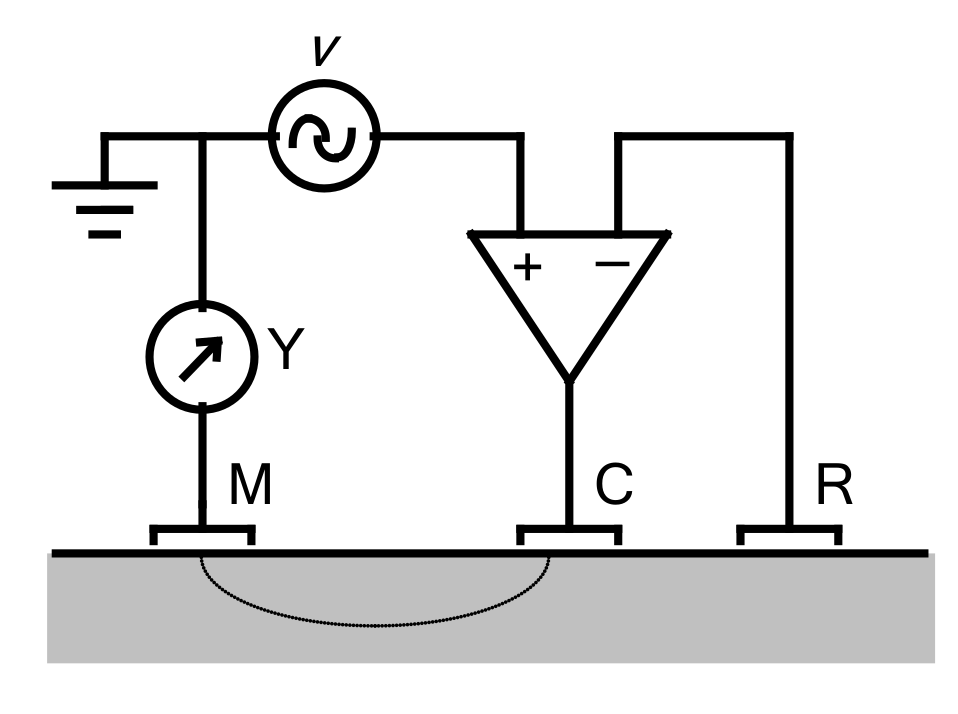
\includegraphics[width = 0.6\textwidth]{fig/screenshot2.png}
\caption{ Tre-elektrodesystem på hud. Hentet fra oppaveteksten.}
\end{figure}

\subsection{Faselåsforsterkeren}
Vi skal benytte oss av en faselåsforsterker for å kunne gjøre nøyaktige målinger i hudens impedans. Dette instrumentet kan låse ut store mengder støy, og plukke ut et enkelt singal med kjent frekvens. Det bygger på prinsippet om at et harmonisk signal er matematisk ortogonalt på alle andre harmoniske signaler med annen frekvens, i form av at et produkt av de to signalene vil bli 0 dersom de ikke har samme frekvens. Instrumentet amplifiserer input signalet, og multipliserer outputen med et referansesignal med samme frekvens som signalet vi skal studere. Dette gir et DC signal proporsjonalt med amplituden til inputsignalet i frekvensområdet til referansesignalet. Faselåsforsterkeren er beskrevet i større detalj i \cite{SR830}



\section{Implementasjon og oppsett}

\subsection{Utstyrsliste}
\begin{itemize}
\item Sølv/sølvklorid-elektroder
\item Multimeter
\item Faselåsforsterker
\item Oscilloskop
\item EKG-monitor
\item Testperson
\end{itemize}

\subsection{Måling av admittans i huden}
For å kontrollere feilkilden introdusert av elektrones impedansovergang fester vi elektrodene direkte mot hverandre. Vi får da bidraget til to elektroder i serie. Vi leser av potensialforskjellen med et multimeter.

For å måle potensialforskjellen mellom to punkter på armen, fester vi en elektrode i håndflaten og en på overarmen. Vi leser av potensialendringen ved forskjellige ytre omstendigheter. Testpersonen ble utsatt for både perioder med ro, og stort ytre stress, inkludert youtubevideoer av edderkopper og hamring i hodet med et oppgavesett. Vi ser også etter polariteten til potensialet.

Vi fester begge elektrodene i håndflaten, og kobler til en faselåsforsterkeren og oscilloskop. Vi leser av admittansen i sanntid fra oscilloskopet, og studerer forskjellen fra resultatene vi observerte når den ene elektroden var festet i armen. Faselåsforsterkeren deler også signalet i real og kompleks del, så vi kan studere konduktansen og suseptansen.

Vi plasserer elektrodene på hver sin underarm, for å studere admittansen gjennom hele 
overkroppen ved forskjellige frekvenser.

\subsection{Måling av hjerterytme - EKG}
Elektrodene forblir på hver sin underarm, og vi setter på en til på den ene armen. Vi kobler nå elektrodene til EKG-monitoren for å studere hjerterytme. For å studere endring i hjertefrekvens, gjennomfører testpersonen fysisk aktivitet i form av knebøy, samt betydelige mengder ytre stress gjennom mobbing fra medstudenter.

\subsection{Måling av muskelspenning - elektromyografi}
Vi flytter referanseelektroden over på sin egen arm, slik at hjerterytmen ikke lenger måles, og vi kan studere muskelspenninger i den andre armen. Dette gjøres ved å henholdsvis slappe av og stramme til musklene i forarmen, og studere frekvens og amplitude på signalet.

\section{Resultater}
\subsection{Måling av admittans i huden}
Vi fant egenpotensialet til elektrodene til å være $\SI{0.4}{mV}$. Dette falt noe ved utsettelse for trykk og temperatur, til $\SI{0.2}{mV}$ ved sitt laveste.

Vi fant en potensialforskjell fra håndflate til underarm på $\SI{33.3}{mV}$ under normale omstendigheter. Etter 30 sekunder med avslapping økte dette til $\SI{37}{mV}$. Ved ytre stress falt potensialforskjellen helt til $\SI{4}{mV}$. Vi så innimellom også negative verdier, som åpenbart ikke er mulig, ettersom spenningen ikke skal kunne bli lavere enn egenpotensialet til elektrodene.

Vi ser at egenpotensialet til elektrodene er betydelig mindre enn verdiene vi måler, og det representerer en liten feilkilde.

Vi klarte ikke å fremkalle noen form for bølger ved tilkobling av faselåsforsterkeren (se \ref{fig:picture1}). Vi syntes dette var merkelig, ettersom vi klarte å fremkalle betydelige endringer i spenningen når vi hadde multimeteret tilkoblet. Etter en stund opplevde vi også at admittansen begynte å stige lineært, uten at våre ytre påvirkninger virket å ha noen effekt.
\begin{figure}[H]
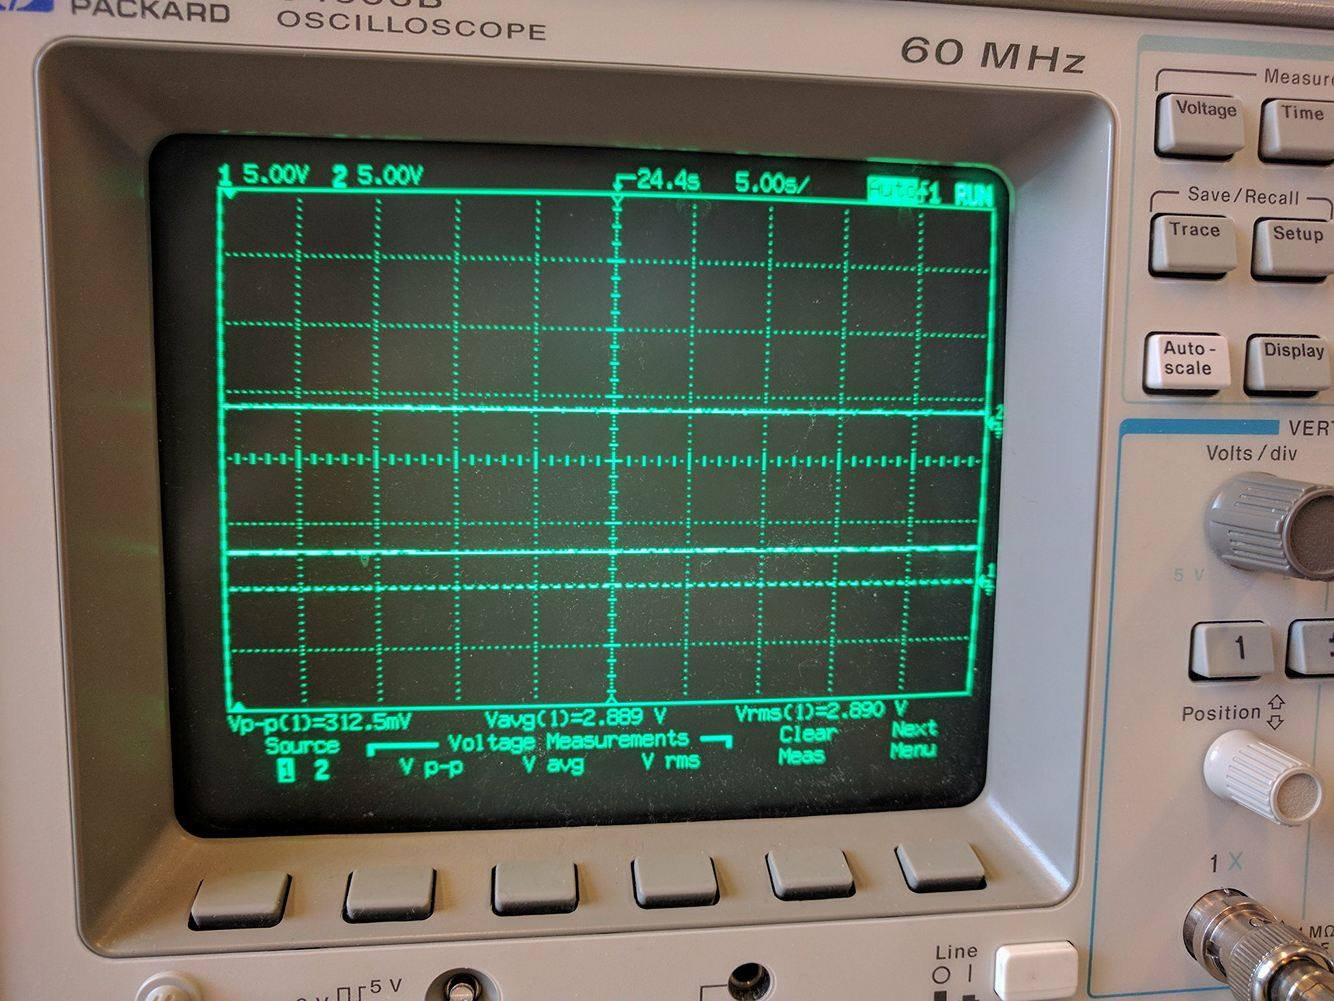
\includegraphics[width = 0.5\textwidth]{fig/picture2.jpg}
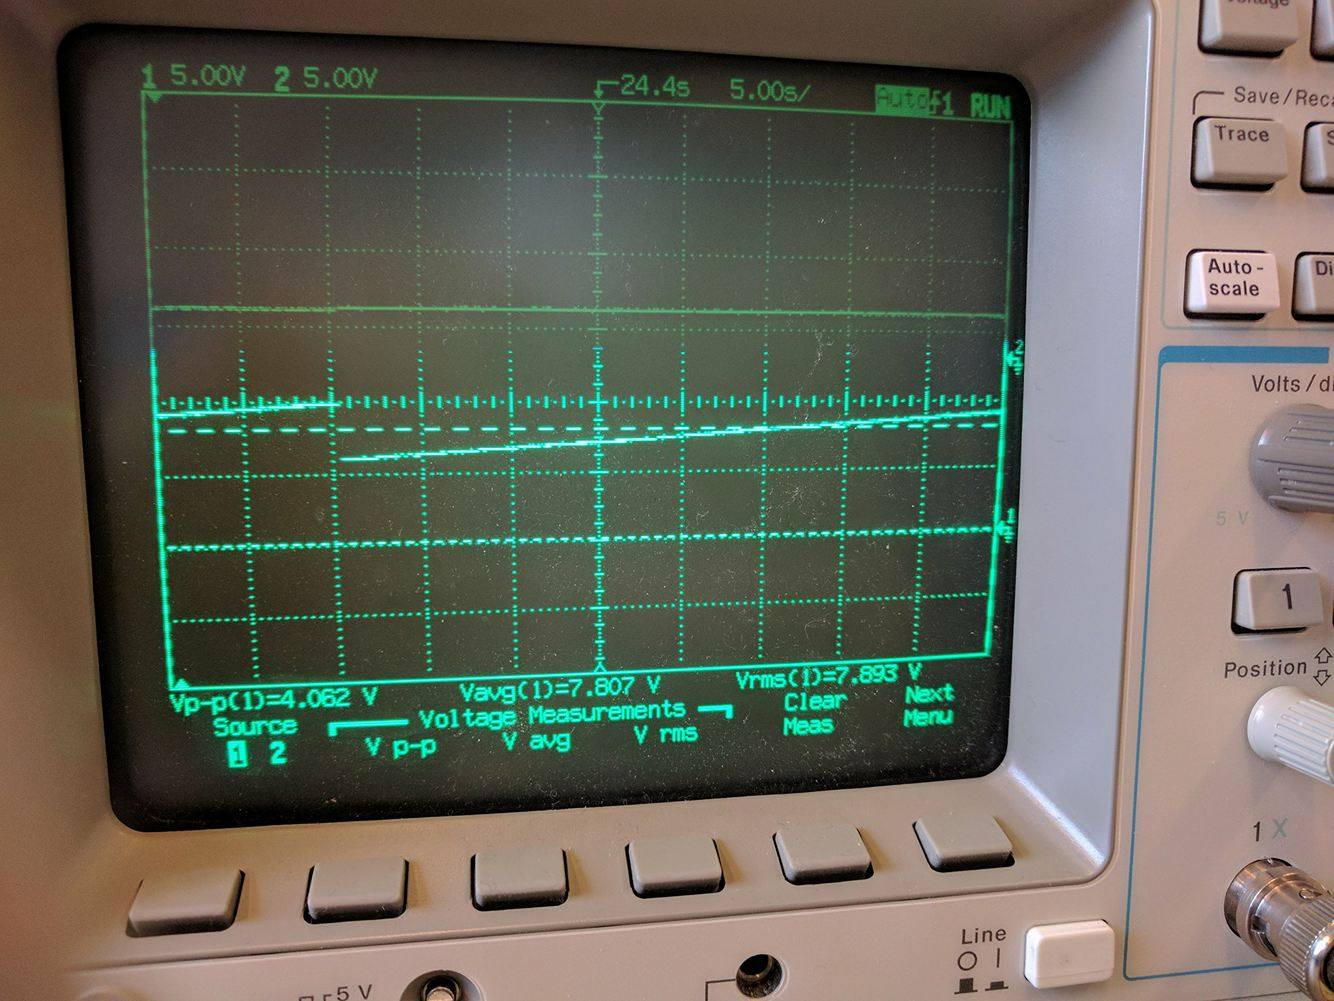
\includegraphics[width = 0.5\textwidth]{fig/picture1.jpg}
\caption{Osciloskop, måling av admittans}
\label{fig:picture1}
\end{figure}

Våre målinger av admittansen over forskjellige frekvenser viser at den ikke forandrer seg spesielt mye. Som vi ser i \ref{fig:admittance} kommer dette enda tydeligere frem i et logaritmisk plot, der den virker tilnærmet konstant. Alle frekvensene er under 10kHz, og vi vet at i dette området kommer admittansen utelukkende fra hornhuden. Hadde vi gått over 10 kHz i frekvens hadde vi nådd den levende huden, og sett forandringer i admittansen. 
\\

\begin{center}
\begin{tabular}{| c | c | c | c | c |}
\hline
Frekvens & Admittans & Fasevinkel & Konduktans & Suseptans \\
$\text{[Hertz]}$ & [$\mu$ Siemens] & [Grader] & [$\mu$ Siemens] & [$\mu$ Siemens] \\
\hline
1 	& 69 & 33 & 58    & 38 \\
10 	& 66 & 32 & 56    & 36 \\
100 	& 73 & 34 & 60    & 41 \\
1000 	& 78 & 35 & 62    & 48 \\
\hline
\end{tabular}
\end{center}

\begin{figure}[H]
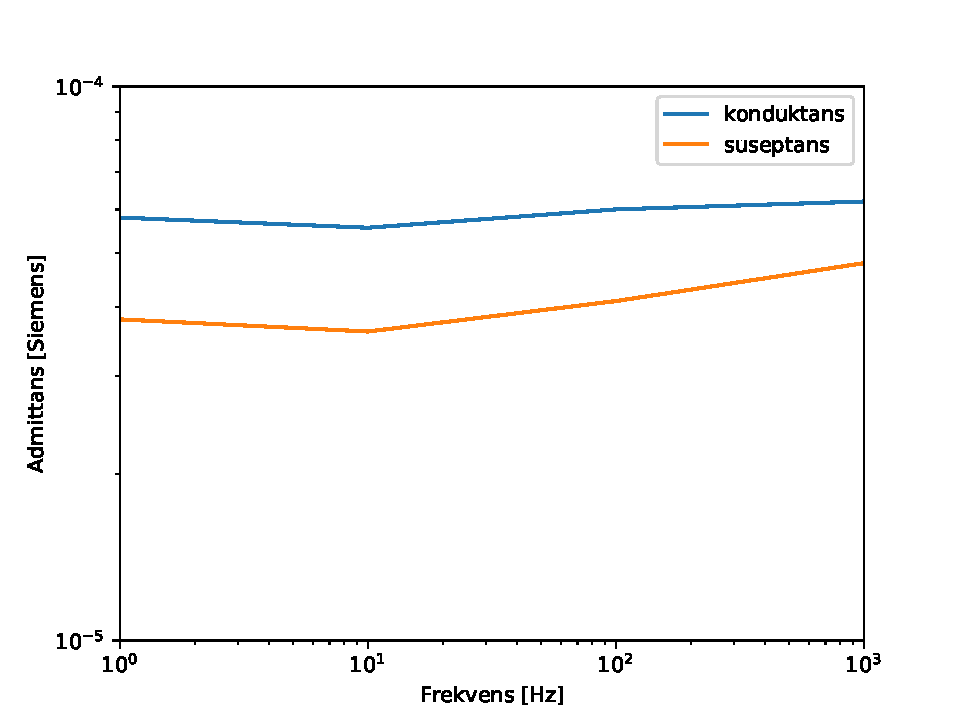
\includegraphics[width = \textwidth]{fig/admittance.pdf}
\caption{Admittans som funksjon av frekvens.}
\label{fig:admittance}
\end{figure}


\subsection{Måling av hjerterytme}
Vi finner at den røde og den gule elektroden plukker opp biopotensialforskjellen, mens den sorte elektroden er referanse. Den gule og røde må være på hver sin arm fordi vi måler potensialendringene gjennom hjertet. 

Fra \ref{fig:picture3} ser vi at testpersonen har en hjertefrekvens på 62 slag per minutt. Vi ser også at amplituden er lik referansefirkantpulsene som ligger på 20.5. En annen testperson hadde betydelig lavere amplitude, som kan skyldes...

\ref{fig:heartrate} viser utviklingen av hjerterytmen over en treningsøkt. Som forventet stiger den kraftig under trening, og synker etter avslutning.

\begin{figure}[H]
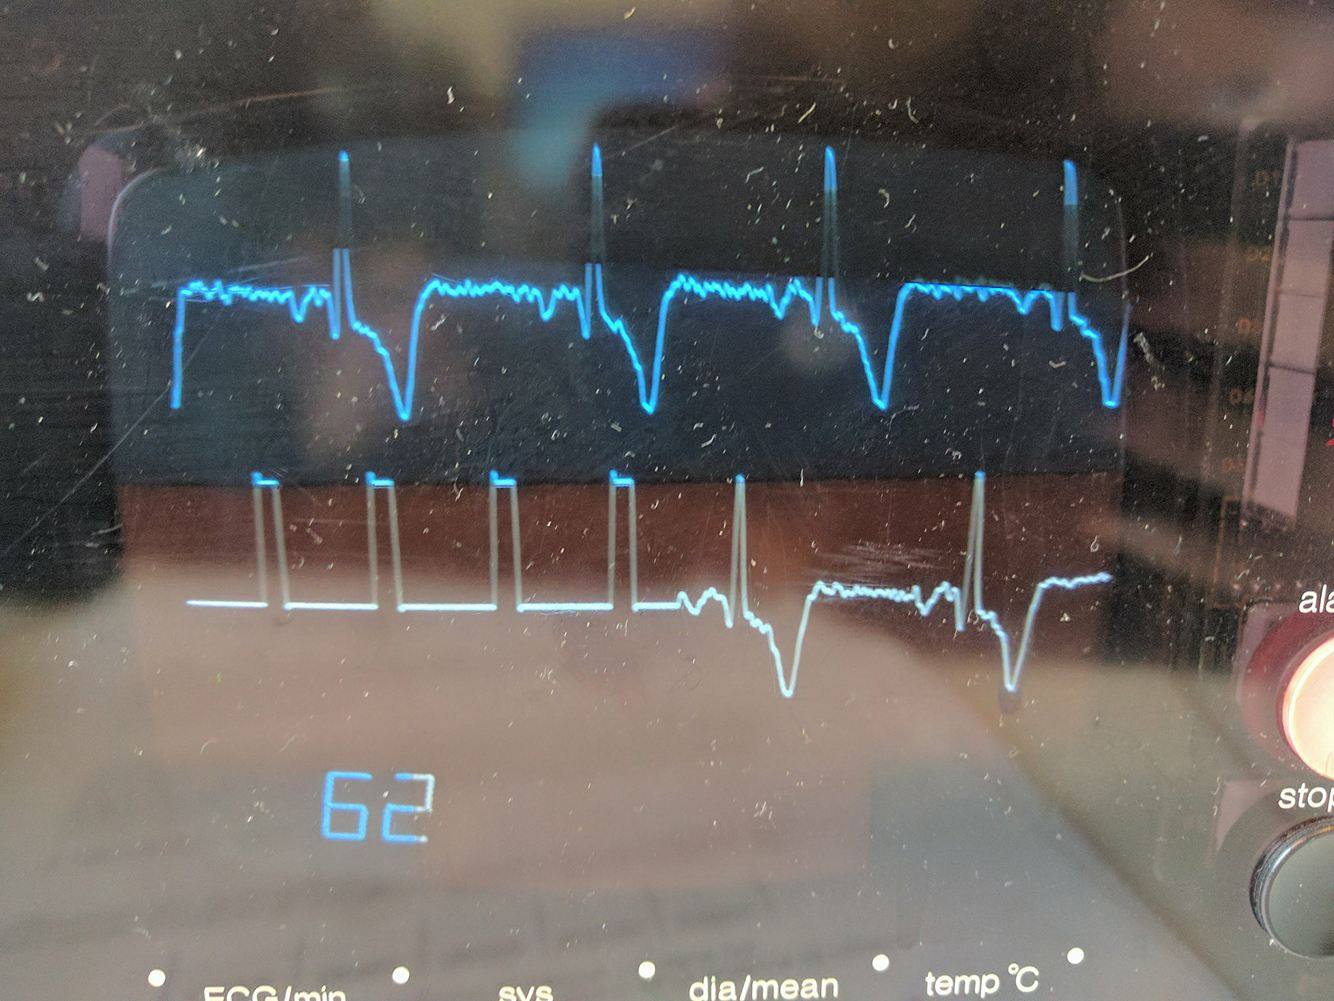
\includegraphics[width = \textwidth]{fig/picture3.jpg}
\caption{Puls over tid.}
\label{fig:picture3}
\end{figure}

\begin{figure}[H]
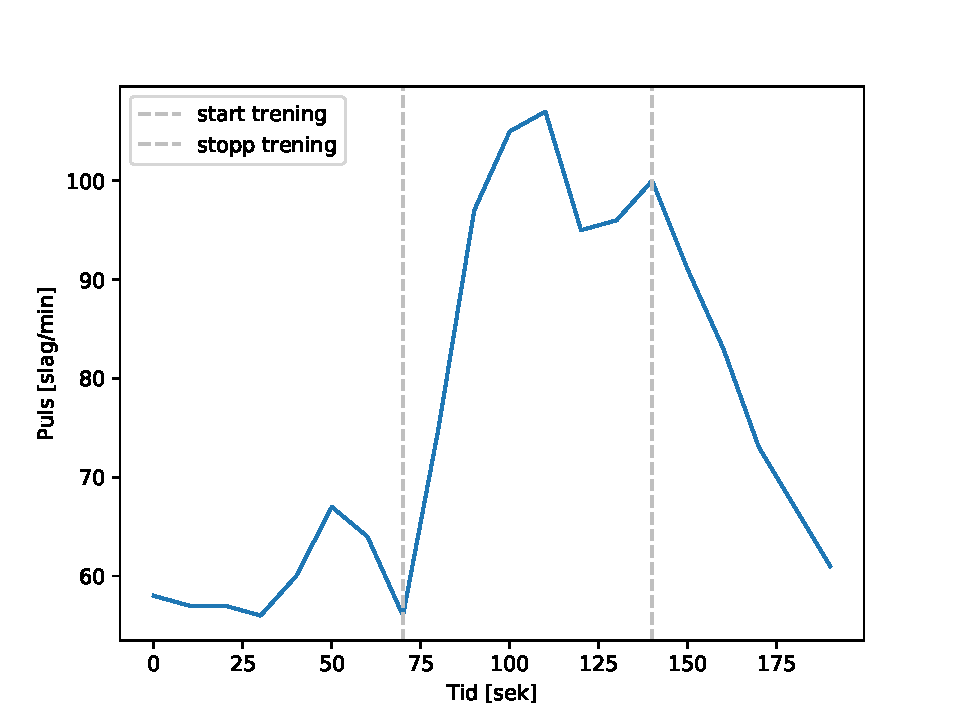
\includegraphics[width = \textwidth]{fig/heartrate.pdf}
\caption{Puls over tid.}
\label{fig:heartrate}
\end{figure}



\subsection{Måling av elektromygografi}
Vi målte 3 sekunder med muskelspenning, og tok et bilde av oscillasjonene i spenningen i denne perioden. Det er ekstremt vanskelig å lese av periodene på bildet, men vi estimerer et sted mellom 100 og 150 perioder i løpet av de 3 sekundene. Dette gir en frekvens i intervallet $f \in [100,\ 150] / 3\,\mathrm{s} = [33, 50]\,\mathrm{Hz}$.

Frekvensen ligger innenfor frekvensdiagrammet vist på side 321 i \cite{MedIns}.

Amplituden varierer en del, men virker å være rundt $A \in [2,\ 7]$, ved sammenligning med referanseamplituden fra firkantpulsene.


\begin{figure}[H]
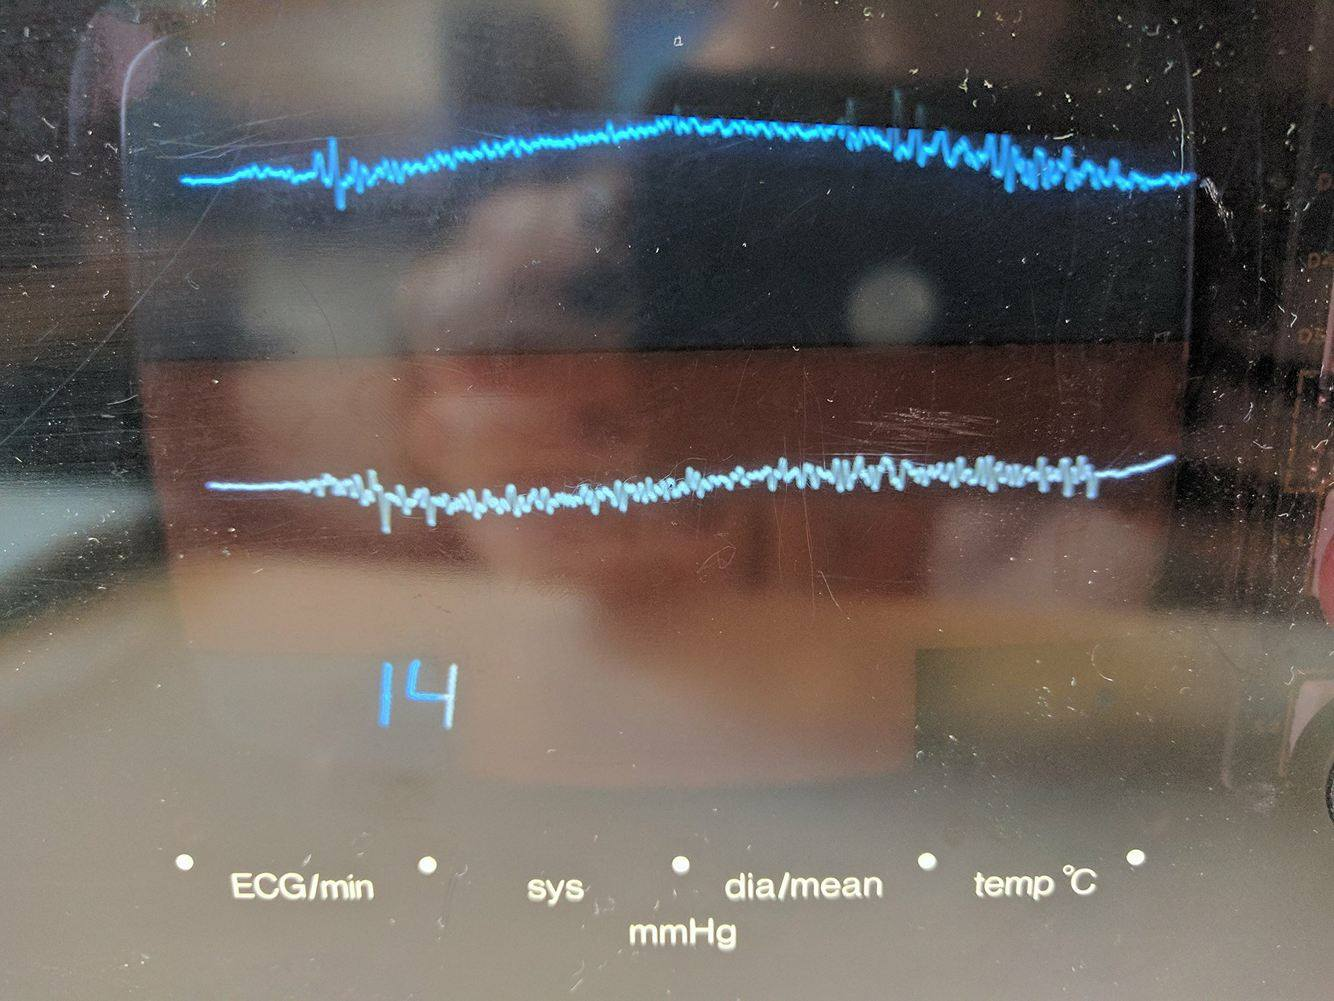
\includegraphics[width = \textwidth]{fig/picture4.jpg}
\caption{Oscilasjoner ved muskelspenning.}
\label{fig:picture4}
\end{figure}

\section{Konklusjon}
Vi har sett at vi kan bruke potensialforskjeller mellom ulike deler av kroppen til å studere hjerterytmer og muskelspenninger, samt hvordan kroppens ledningsevne blir påvirket både av fysisk og psykisk stimuli. Vi har erfart at det er store feilkilder og støykilder involvert i elektrisk arbeid med organisk materiale.



\begin{thebibliography}{9}

\bibitem{SR830}
    Stanford Research Systems,
    \emph{Model SR830, DPS Lock-In Amplifier},
    Revision 2.5,
    2011,
    \url{http://www.thinksrs.com/downloads/PDFs/Manuals/SR830m.pdf}.

\bibitem{BioImp}
    Sverre Grimnes og Ørjan Grøttem Martinsen,
    \emph{Bioimpedance and Bioelectricity Basics},
    Academic Press

\bibitem{MedIns}
    John G. Webster,
    \emph{Medical Instrumentation - Application and Design},
    Second edition

\end{thebibliography}











\end{document}


